%%% LaTeX Template: Designer's CV
%%%
%%% Source: http://www.howtotex.com/
%%% Feel free to distribute this template, but please keep the referal to HowToTeX.com.
%%% Date: March 2012


%%%%%%%%%%%%%%%%%%%%%%%%%%%%%%%%%%%%%
% Document properties and packages
%%%%%%%%%%%%%%%%%%%%%%%%%%%%%%%%%%%%%
\documentclass[a4paper,12pt,final]{memoir}

% misc
\renewcommand{\familydefault}{bch}	% font
\pagestyle{empty}					% no pagenumbering
\setlength{\parindent}{0pt}			% no paragraph indentation


% required packages (add your own)
\usepackage{flowfram}										% column layout
\usepackage[top=1cm,left=1cm,right=1cm,bottom=1cm]{geometry}% margins
\usepackage{graphicx}										% figures
\usepackage{url}											% URLs
\usepackage[usenames,dvipsnames]{xcolor}					% color
\usepackage{multicol}										% columns env.
	\setlength{\multicolsep}{0pt}
\usepackage{paralist}										% compact lists
\usepackage{hyperref}										% External Links
\usepackage{tikz}

%%%%%%%%%%%%%%%%%%%%%%%%%%%%%%%%%%%%%
% Links customization
%%%%%%%%%%%%%%%%%%%%%%%%%%%%%%%%%%%%%
\hypersetup{
    colorlinks=true,
    urlcolor=blue,
}

%%%%%%%%%%%%%%%%%%%%%%%%%%%%%%%%%%%%%
% Create column layout
%%%%%%%%%%%%%%%%%%%%%%%%%%%%%%%%%%%%%
% define length commands
\setlength{\vcolumnsep}{\baselineskip}
\setlength{\columnsep}{\vcolumnsep}

% frame setup (flowfram package)
% left frame
\newflowframe{0.2\textwidth}{\textheight}{0pt}{0pt}[left]
	\newlength{\LeftMainSep}
	\setlength{\LeftMainSep}{0.2\textwidth}
	\addtolength{\LeftMainSep}{1\columnsep}
 
% small static frame for the vertical line
\newstaticframe{1.5pt}{\textheight}{\LeftMainSep}{0pt}
 
% content of the static frame
\begin{staticcontents}{1}
\hfill
\tikz{%
	\draw[loosely dotted,color=RoyalBlue,line width=1.5pt,yshift=0]
	(0,0) -- (0,\textheight);}%
\hfill\mbox{}
\end{staticcontents}
 
% right frame
\addtolength{\LeftMainSep}{1.5pt}
\addtolength{\LeftMainSep}{1\columnsep}
\newflowframe{0.7\textwidth}{\textheight}{\LeftMainSep}{0pt}[main01]


%%%%%%%%%%%%%%%%%%%%%%%%%%%%%%%%%%%%%
% define macros (for convience)
%%%%%%%%%%%%%%%%%%%%%%%%%%%%%%%%%%%%%
\newcommand{\Sep}{\vspace{1.5em}}
\newcommand{\SmallSep}{\vspace{0.5em}}

\newenvironment{AboutMe}
	{\ignorespaces\textbf{\color{RoyalBlue} About me}}
	{\Sep\ignorespacesafterend}
	
\newcommand{\CVSection}[1]
	{\Large\textbf{#1}\par
	\SmallSep\normalsize\normalfont}

\newcommand{\CVItem}[1]
	{\textbf{\color{RoyalBlue} #1}}


%%%%%%%%%%%%%%%%%%%%%%%%%%%%%%%%%%%%%
% Begin document
%%%%%%%%%%%%%%%%%%%%%%%%%%%%%%%%%%%%%
\begin{document}

% Left frame
%%%%%%%%%%%%%%%%%%%%
\begin{figure}
	\hfill
	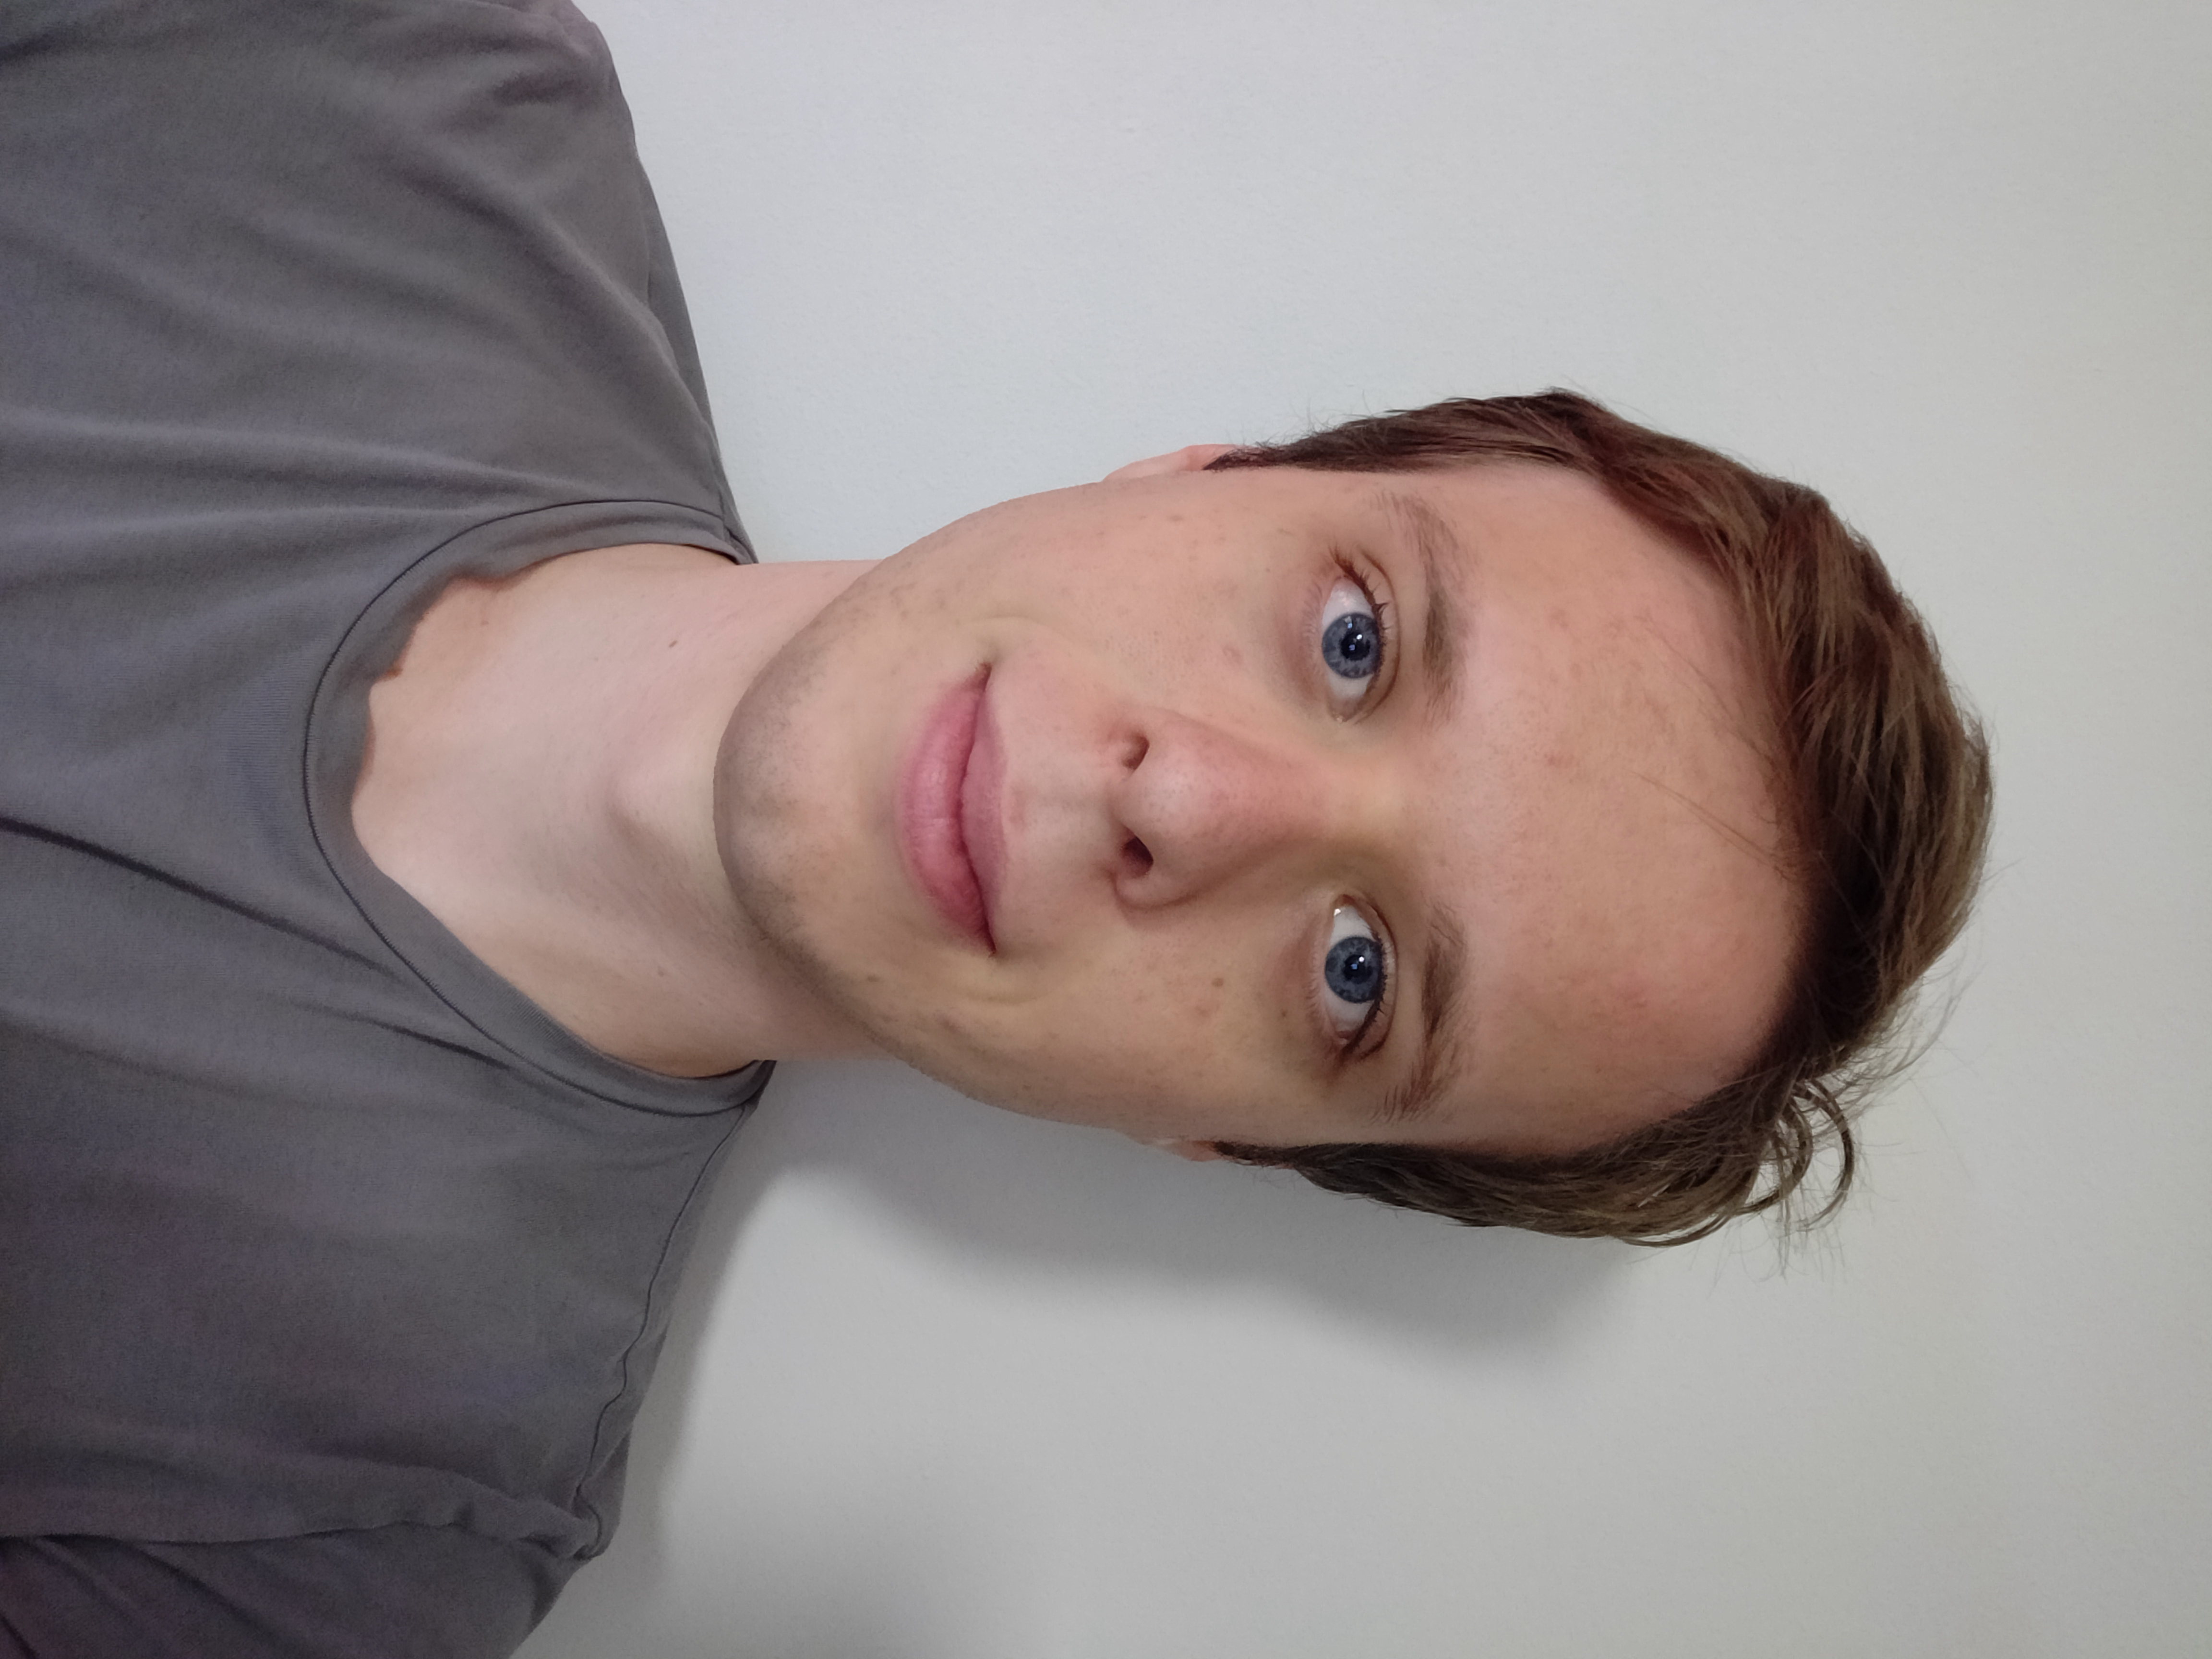
\includegraphics[width=1\columnwidth, angle=90]{photo-Mattia}
	\vspace{-7cm}
\end{figure}

\begin{flushright}\small
	Mattia Rubini \\
	mattia.rubini@gmail.com \\
	+39 329 617 1153 \\
	Account: 
	\href{https://github.com/Mot93}{GitHub}\\
	Account:
	\href{https://gitlab.com/mattia.rubini}{GitLab}\\
	Account:
	\href{https://stackoverflow.com/users/6875945/mattia-rubini}{Stack Overflow}
\end{flushright}\normalsize
\framebreak


% Right frame
%%%%%%%%%%%%%%%%%%%%
\Huge\bfseries {\color{RoyalBlue} Rubini Mattia} \\
\Large\bfseries  Developer - Laureando in Ing. Informatica \\

\normalsize\normalfont

% About me
\CVSection{Presentazione}
    Sono un laureando in Ingegneria Informatica all'università di Bologna, e mi dedico a progetti di programmazione dall'età di 14 anni.\\
	In tutto quello che faccio, cerco sempre di migliorarmi e di imparare cose nuove.
	Tutti i progetti realizzati fino ad oggi sono frutto sia del mio lavoro da autodidatta che degli approfondimenti che sto acquisendo nel corso di laurea in Ingegneria Informatica
	(Questo curriculum è stato realizzato con \LaTeX, un linguaggio markup:
	il sorgente si trova su \href{https://github.com/Mot93/CV-Mattia-Rubini}{account gitHub})\\
\Sep


% Experience
\CVSection{Esperienze}
\CVItem{Feb 2017 - Mag 2017, Postfix Calculator (app Android)}\\
	Ho imparato a programmare app usando android studio, Java e XML. 
	A seguire ho pubblicato una app android \href{https://play.google.com/store/apps/details?id=postfixcalculator.mattiarubini.com.postfixcalculator}{ Postifix Calculator}.
	Il codice sorgente è pubblico su \href{https://gitlab.com/mattia.rubini/PostfixCalculator}{gitlab}
\SmallSep

\CVItem{Nov 2016 - Feb 2017, Wordpress (sito personale)}\\
	Ho imparato a fare siti con wordpress. 
	Con queste nozioni ho fatto il mio sito personale. Il codice sorgente è disponibile su \href{https://github.com/Mot93/MattiaRubini-com-wordpress-theme}{github}.
\Sep

% Education
\CVSection{Formazione}

\CVItem{2017 - ad oggi, Laureando in Ingegneria Informatica}\\
	Nel 2017 ho deciso di cambiare facoltà, per focalizzarmi sullo studio dell'informatica, presso l'Alma Mater Studiorum di Bologna.
\SmallSep

\CVItem{2014 - 2015, Borsa di studio a Shanghai}\\
	Vincitore della borsa di studio di Ingegneria per l'overseas di un anno a Shanghai, presso la Tongji University.
\SmallSep

\CVItem{2013 - 2016, Laureando in Ingegneria dell'Automazione}\\
	% Bologna è a capo per non rompere il file
	\textbf{Interrotto, per trasferimento ad Informatica.}\\
	Iscritto presso il corso di laurea di Ingegneria dell'Automazione presso l'Alma Mater Studiorum di Bologna.
	Superati 15 esami. 
\SmallSep

\CVItem{2007 - 2013, Diploma}\\
	Diplomato presso il liceo scientifico Niccolò Copernico di Bologna.\\
	Indirizzo di studi MAXI (potenziamento di liceo scientifico, su materie: matematica, fisica, programmazione e scienze).\\
	Tale indirizzo insegna a programmare fin dai primi anni. 
\Sep

% Skills
\CVSection{Competenze}
\CVItem{Competenze informatiche avanzate}
\begin{multicols}{3}
\begin{compactitem}[\color{RoyalBlue}$\circ$]
	\item Python 
	\item Java
	\item HTML
	\item CSS
	\item git
	\item shell
	\item bash
\end{compactitem}
\end{multicols}
\SmallSep

% reset boundaries when going on a new page
\clearpage
\framebreak
\framebreak

\CVItem{Competenze informatiche}
\begin{multicols}{3}
\begin{compactitem}[\color{RoyalBlue}$\circ$]
	\item Database SQL
	\item Wordpress
	\item Django
	\item \LaTeX
	\item pascal
	\item Windows
	\item Linux
	\item MacOS
	\item raspberry py
	\item arduino
	\item Haskell
	\item Assemblamento\\computer
\end{compactitem}
\end{multicols}
\SmallSep

\CVItem{Lingue conosciute}
\begin{multicols}{3}
\begin{compactitem}[\color{RoyalBlue}$\circ$]
	\item Italiano\\(madrelingua)
	\item Francese\\(madrelingua)
	\item Inglese (avanzato)
\end{compactitem}
\end{multicols}
\Sep 

\CVSection{Motivazione}
	Non mi spavento facilmente davanti le avversità.
	Per non fermarmi davanti il primo ostacolo, a 16 anni ho imparato l'inglese (livello avanzato) per accedere a più materiale possibile.
	\\Inoltre, trovo sempre un modo per risolvere i problemi, come dimostra il mio account \href{https://stackoverflow.com/users/6875945/mattia-rubini}{Stack Overflow}.
	\\Sempre grazie a \href{https://stackoverflow.com/users/6875945/mattia-rubini}{Stack Overflow} ho imparato ad essere chiaro e preciso nella esposizione e risoluzione dei problemi.

\CVSection{Altre esperienze}
	Membro del Rotaract Club Bologna Valle del Savena.
	\\Ho assemblato il mio computer.
	\\In passato ho fatto ampio uso di arduino e il raspberry pi.
	\\Vacanza studio-lavoro di un mese con attività di volontariato per la ripopolazione della vegetazione in Islanda.
	\\Vacanza studio-lavoro di un mese con attività di volontariato per la preparazione di una struttura dedicata a ragazzi disadattati in Inghilterra.
	\\Attività di volontariato presso circolo Ancescao di Corticella in qualità di barista.
	\\Lavoro estivo in qualità di magazziniere in struttura a temperatura controllata, per generi alimentari.
\Sep

% References
%\CVSection{References}
%References upon request.

%%%%%%%%%%%%%%%%%%%%%%%%%%%%%%%%%%%%%
% End document
%%%%%%%%%%%%%%%%%%%%%%%%%%%%%%%%%%%%%
\end{document}